\documentclass[xcolor=dvipsnames]{beamer}
\usepackage{lmodern}
\usepackage[T1]{fontenc}
\usepackage[english]{babel}
\usepackage[utf8]{inputenc}

\usepackage{manfnt}
\usepackage{wasysym}
\usepackage{listings}
\usepackage{graphicx}
\usepackage{url}
\usepackage{ulem}
\usepackage{marvosym}
\usepackage{skull}
\usepackage{proof}
\usepackage{array}
\setbeamertemplate{navigation symbols}{}

\title[Kinds for Parallelism]{{\bf Types of Types in Rust}}
\subtitle[]{ {\em Better parallelism through traits and kinds}}
\author[Ben Blum]{Ben Blum \texttt{(bblum@andrew.cmu.edu)}}

\institute[Mozilla Research]{Mozilla Research}
\date[]{2013, August 13}

\setbeamertemplate{footline}{\hspace*{.5cm}\scriptsize{\insertauthor\hspace*{50pt} \hfill\insertframenumber\hspace*{.5cm}}} 

\usecolortheme{seahorse}
\usecolortheme{rose}
\useoutertheme{infolines}

\usecolortheme[named=RoyalBlue]{structure}

\newcommand\noob{\mathsf{noob}}
\newcommand\gibs{\mathsf{gibs}}
\newcommand\dps{\mathsf{dps}}
\newcommand\squig\rightsquigarrow
\newcommand\Coloneqq{\mathrel{\mathop{::}}=}
\newcommand\dmg{\text{\Laserbeam}}
\newcommand\delter\delta
\newcommand\alpher\alpha
\newcommand\defnor{\text{ }|\text{ }}

\newcommand\pimp{\mathop{\supset}}
\newcommand\pand{\mathop{\wedge}}
\newcommand\por{\mathop{\vee}}
\newcommand\ptrue{\top}
\newcommand\pfalse{\bot}


\begin{document}
\renewcommand{\inserttotalframenumber}{28}
\normalem
\begin{frame}
	\titlepage
\end{frame}

%%%%%%%%%%%%%%%%%%%%%%%%%%%%%%%%%%%%%%%%%%%%%%%%%%%%%%%%%%%%%%%%%%%%%%%%%%%%%%%%
%%%%%%%%%%%%%%%%%%%%%%%%%%%%%%%%%%%%%%%%%%%%%%%%%%%%%%%%%%%%%%%%%%%%%%%%%%%%%%%%
%%%%%%%%%%%%%%%%%%%%%%%%%%%%%%%%%%%%%%%%%%%%%%%%%%%%%%%%%%%%%%%%%%%%%%%%%%%%%%%%

\newcommand\linegap{\vspace{0.2in}}
\newcommand\breakslide[1]{\begin{frame}{} \begin{center} \Large #1 \end{center} \end{frame}}
\newcommand\related[1]{\textsuperscript{\em [#1]}}
\newcommand\hilight[2]{\color{#1}#2\color{black}}

\begin{frame}{Outline}
	\begin{columns}
	\column{0.05\textwidth}
	\column{0.5\textwidth}
	\textbf{Overview}
	\begin{itemize}
		\item Kinds Overview
		\item Traits Overview
		\item Existential Types Overview
	\end{itemize}
	\linegap

	{\bf Kind Bounds}
	\begin{itemize}
		\item Reasoning about Captures
		\item New Expressivity
	\end{itemize}
	\linegap

	{\bf Use Case: Concurrent Data Structures}
	\linegap

	\column{0.45\textwidth}
	\begin{center}
	
\includegraphics[width=0.9\textwidth]{rust.png}
	\end{center}
	\end{columns}
\end{frame}

\begin{frame}{We have a new runtime!}
	I also worked on it, but... \\
	\pause
	\begin{center}
		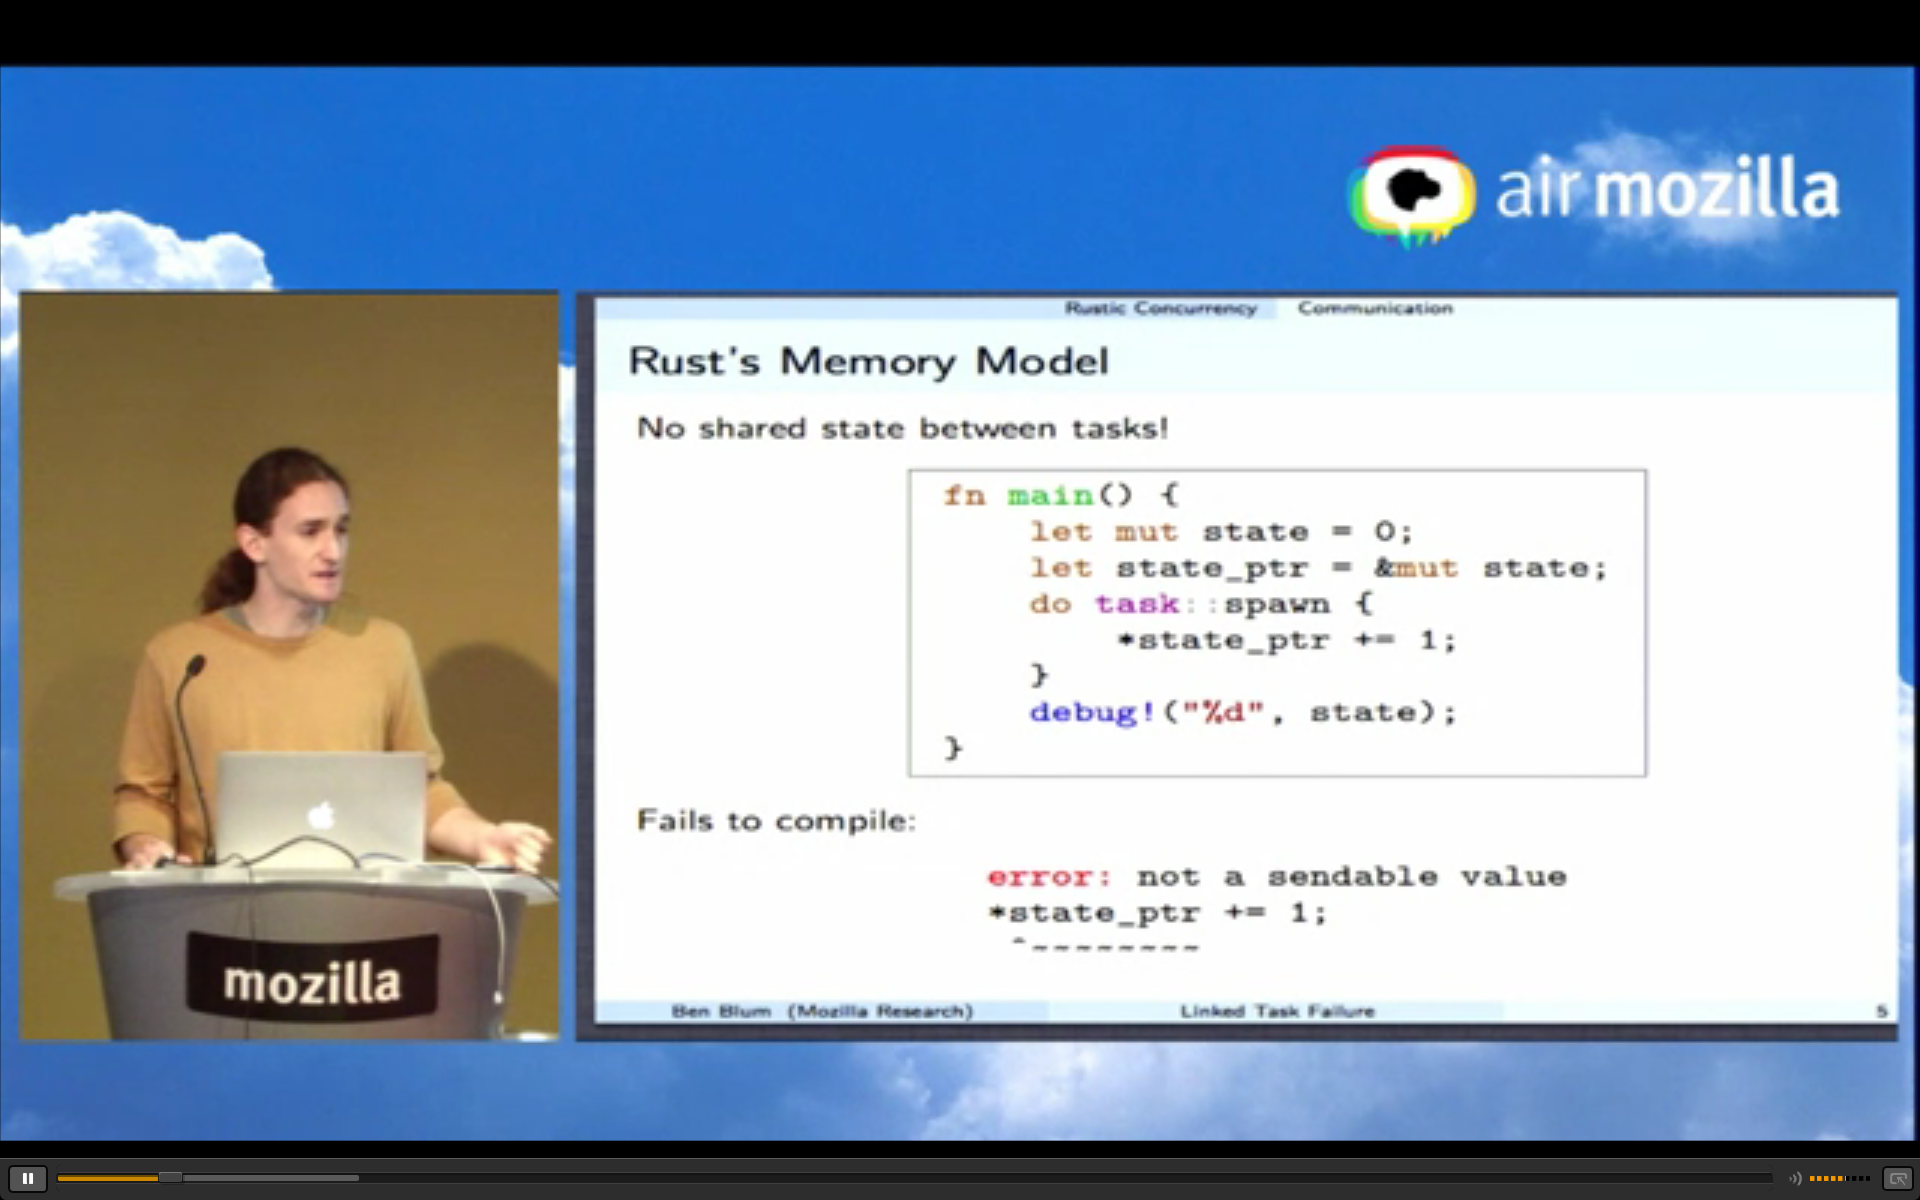
\includegraphics[width=0.8\textwidth]{last-year.png}
	\end{center}
\end{frame}

%%%%%%%%%%%%%%%%%%%%%%%%%%%%%%%%%%%%%%%%%%%%%%%%%%%%%%%%%%%%%%%%%%%%%%%%%%%%%%%%
\section{Overview}
%%%%%%%%%%%%%%%%%%%%%%%%%%%%%%%%%%%%%%%%%%%%%%%%%%%%%%%%%%%%%%%%%%%%%%%%%%%%%%%%

\newcommand\code[1]{{\begin{center}\fbox{\begin{tabular}{l} #1 \end{tabular}} \end{center}}}

\definecolor{grey}{RGB}{127,127,127}
\definecolor{darkcyan}{RGB}{0,127,127}
\definecolor{olivegreen}{RGB}{0,127,0}
\definecolor{violet}{RGB}{127,0,127}
\definecolor{brickred}{RGB}{127,0,0}
\definecolor{brown}{RGB}{127,63,0}

\breakslide{Kinds}

\subsection{Kinds Overview}

\begin{frame}{What are Kinds?}
	\begin{itemize}
		\item Type theory lingo: ``kinds'' == ``types of types''
		\pause
		\item In Rust, kinds (aka ``builtin bounds'') describe {\em capabilities} of types:
		\begin{itemize}
			\item {\tt \hilight{violet}{Send}} - Data can be sent to other tasks
			\item {\tt \hilight{violet}{Freeze}} - Data has no mutable interior
			\item {\tt \hilight{violet}{Static}} - Data never goes out of scope
			\item {\tt \hilight{violet}{Copy}} - Data can be implicitly copied
				\pause
				\begin{itemize}
					\item $\skull$
				\end{itemize}
		\end{itemize}
		\pause
		\item Kind bounds are automatically derived: \\
		\begin{itemize}
			\item \begin{tabular}{l}
				\texttt{\hilight{brown}{enum}~\hilight{olivegreen}{Option}<T>~\{} \\
				\texttt{~~~~\hilight{brickred}{Some}(T),} \\
				\texttt{~~~~\hilight{brickred}{None}} \\
				\texttt{\}} \\
			\end{tabular}
		\item {\tt \hilight{olivegreen}{Option}<T>} has kind {\tt \hilight{violet}{K}} iff {\tt T} has kind {\tt \hilight{violet}{K}}.
		\end{itemize}
	\end{itemize}
\end{frame}

\subsection{Motivation}
\begin{frame}{What are kind bounds good for?}
		Message passing:
		\begin{itemize}
			\item \begin{tabular}{l}
					\texttt{\hilight{brown}{fn}~stream<T:~\hilight{violet}{Send}>()~->~(\hilight{olivegreen}{Port}<T>,~\hilight{olivegreen}{Chan}<T>)} \\
					\texttt{} \\
					\texttt{\hilight{brown}{fn}~recv<T:~\hilight{violet}{Send}>(port:~\&\hilight{olivegreen}{Port}<T>)~->~T} \\ 
					\texttt{} \\
					\texttt{\hilight{brown}{fn}~send<T:~\hilight{violet}{Send}>(chan:~\&\hilight{olivegreen}{Chan}<T>,~data:~T)} \\

			\end{tabular}
			\pause
			\linegap
			\item \texttt{\hilight{violet}{Send}} bound ensures once data is sent, sender can no longer access it.
		\end{itemize}
\end{frame}
\begin{frame}{What are kind bounds good for?}
		Shared state across tasks:
		\begin{itemize}
			\item \begin{tabular}{l}
					\texttt{\hilight{brown}{fn}~arc<T:~\hilight{violet}{Send}+\hilight{violet}{Freeze}>(data:~T)~->~\hilight{olivegreen}{Arc}<T>} \\
					\\
					\texttt{\hilight{brown}{fn}~clone<T:~\hilight{violet}{Send}+\hilight{violet}{Freeze}>(arc:~\&\hilight{olivegreen}{Arc}<T>)~->~\hilight{olivegreen}{Arc}<T>} \\
					\texttt{} \\
					\texttt{\hilight{darkcyan}{//~note~immutable~pointer~to~T}} \\
					\texttt{\hilight{brown}{fn}~get<'a,~T:~\hilight{violet}{Send}+\hilight{violet}{Freeze}>(arc:~\&'a~\hilight{olivegreen}{Arc}<T>)~->~\&'a~T} \\

			\end{tabular}
			\pause
			\linegap
		\item \texttt{\hilight{violet}{Send}} bound ensures only way to access data is through the \texttt{\hilight{olivegreen}{Arc}}
		\item \texttt{\hilight{violet}{Freeze}} bound ensures data is immutable
		\end{itemize}
\end{frame}

\subsection{Traits Overview}
\breakslide{Traits and Objects}

\begin{frame}{What are Traits?}
	\begin{itemize}
		\item Typeclasses, interfaces, ...
			\begin{itemize}
				\item \begin{tabular}{l}
						\texttt{\hilight{brown}{trait}~\hilight{olivegreen}{Pet}~\{} \\

							\texttt{~~~~\hilight{brown}{fn}~name(\&self)~->~\textasciitilde{}\hilight{olivegreen}{str}} \\
							\texttt{~~~~\hilight{brown}{fn}~num\_legs(\&self)~->~\hilight{olivegreen}{int}} \\
							\texttt{~~~~\hilight{brown}{fn}~is\_well\_behaved(\&self)~->~\hilight{olivegreen}{bool}} \\
					\texttt{\}} \\

				\end{tabular}
			\end{itemize}
		\pause
		\item Also objects (existential types):
			\begin{itemize}
				\item \begin{tabular}{l}
						\texttt{struct~\hilight{olivegreen}{Dog}~\{~name:~\textasciitilde{}\hilight{olivegreen}{str},~bark\_decibels:~\hilight{olivegreen}{int}~\}} \\
					\texttt{} \\
					\texttt{\hilight{brown}{impl}~\hilight{olivegreen}{Pet}~\hilight{brown}{for}~\hilight{olivegreen}{Dog}~\{~...~\}} \\
					\texttt{} \\
					\texttt{\hilight{brown}{let}~alan\_turing:~\hilight{olivegreen}{Dog}~=~\hilight{olivegreen}{Dog}~\{~...~\}} \\
					\texttt{} \\
					\texttt{\hilight{brown}{let}~generic\_pet:~\&\hilight{olivegreen}{Pet}~=~\&alan\_turing~\hilight{brown}{as}~\&\hilight{olivegreen}{Pet};} \\
					\texttt{~~~~\hilight{darkcyan}{//~\^~value~contains~a~vtable}} \\

				\end{tabular}
			\end{itemize}
	\end{itemize}
\end{frame}

\begin{frame}{Existential Types}
	\begin{itemize}
		\item ``Opaque type that presents a generic interface''
		\begin{itemize}
			\item $\exists x:T \rightarrow \mathsf{SomeInterface}(x)$
		\end{itemize}
		\item OOP: Interfaces-as-objects
		\pause
		\item Closures are a ``special case'' of trait objects:
		\begin{itemize}
			\item \begin{tabular}{l}
					\texttt{\hilight{brown}{trait}~\hilight{olivegreen}{Closure}<Args,Ret>~\{} \\
			\texttt{~~~~\hilight{brown}{fn}~call(self,~Args)~->~Ret;} \\
			\texttt{\}} \\
			\end{tabular}
		\end{itemize}
		\pause
		\item In Rust, existential objects are {\em dynamically-sized}
			\begin{itemize}
				\item Have to be hidden behind a {\tt \&}, {\tt \textasciitilde}, or {\tt @} pointer.
			\end{itemize}

	\end{itemize}
\end{frame}

\begin{frame}{What's in an Object?}
	\begin{itemize}
		\item (In terms of kind bounds?)
		\pause
		\item Some inflexible defaults:
			\begin{itemize}
				\item {\tt \textasciitilde{}\hilight{olivegreen}{Trait}} can only contain {\tt \hilight{violet}{Send}}able values
				\item {\tt @\hilight{olivegreen}{Trait}} can only contain {\tt \hilight{violet}{Static}} values
				\item {\tt \&\hilight{olivegreen}{Trait}} can contain any values
				\pause
				\item Traits are not {\tt \hilight{violet}{Freeze}}able or {\tt \hilight{violet}{Copy}}able.
			\end{itemize}
			\pause
		\item Enter {\em kind bounds}.
	\end{itemize}
\end{frame}

\section{Kind Bounds}
\breakslide{Kind Bounds}

\subsection{Reasoning about Captured Values}

\begin{frame}{Kind Bounds on Traits}
	\begin{itemize}
		\item Today, \texttt{\textasciitilde{}\hilight{olivegreen}{Pet}:\hilight{violet}{Copy}} is also a type.

		\begin{itemize}
			\item Restriction: ``Only copyable values can be captured in this``
			\item Capability: ``...so this whole thing can be copied!''
		\end{itemize}
		\pause
		Example:
		\begin{itemize}
			\item \begin{tabular}{l}
				\texttt{\hilight{brown}{let}~noncopyable\_alan\_turing:~\hilight{olivegreen}{Dog}~=~\hilight{olivegreen}{Dog}~\{~...~\}} \\
				\pause
				\texttt{} \\
				\texttt{\hilight{brown}{let}~generic\_pet:~\&\hilight{olivegreen}{Pet}~=~\&noncopyable\_alan\_turing~\hilight{brown}{as}~\&\hilight{olivegreen}{Pet};} \\
				\texttt{~~~~\hilight{darkcyan}{//~\^~OK}} \\
				\texttt{} \\
			\texttt{\hilight{brown}{let}~copyable\_pet:~\&\hilight{olivegreen}{Pet}:\hilight{violet}{Copy}~=} \\
				\texttt{~~~~~~~~\&noncopyable\_alan\_turing~\hilight{brown}{as}~\&\hilight{olivegreen}{Pet}:\hilight{violet}{Copy};} \\
				\texttt{~~~~\hilight{darkcyan}{//~\^~{error}:~cannot~capture~noncopyable}} \\
				\texttt{~~~~\hilight{darkcyan}{//~~~~~~~~~~~value~in~{trait}~bounded~by~{Copy}}} \\
			\end{tabular}
		\end{itemize}
	\end{itemize}
\end{frame}

\begin{frame}{What is this good for?}
	\begin{itemize}
		\item {\bf Sharing lists of objects between threads}
		\pause
		\begin{itemize}
			\item ``Heterogeneous'' objects, i.e., different implementations of the same trait
		\end{itemize}
		\pause
		Example:
		\begin{itemize}
			\item \begin{tabular}{l}
					\texttt{\hilight{brown}{let}~alan\_turing~=~\textasciitilde{}\hilight{olivegreen}{Dog}~\{~...~\}} \\
					\texttt{\hilight{brown}{let}~ada\_lovelace~=~\textasciitilde{}\hilight{olivegreen}{Cat}~\{~...~\}} \\
					\texttt{\hilight{brown}{let}~albert\_einstein~=~\textasciitilde{}\hilight{olivegreen}{Bird}~\{~...~\}} \\
					\pause
					\texttt{}\\
					\texttt{\hilight{brown}{let}~pets~=~\textasciitilde{}[alan\_turing~~~~~\hilight{brown}{as}~\textasciitilde{}\hilight{olivegreen}{Pet}:~\hilight{violet}{Send}+\hilight{violet}{Freeze},} \\
						\texttt{~~~~~~~~~~~~~ada\_lovelace~~~~\hilight{brown}{as}~\textasciitilde{}\hilight{olivegreen}{Pet}:~\hilight{violet}{Send}+\hilight{violet}{Freeze},} \\
					\texttt{~~~~~~~~~~~~~albert\_einstein~\hilight{brown}{as}~\textasciitilde{}\hilight{olivegreen}{Pet}:~\hilight{violet}{Send}+\hilight{violet}{Freeze}];} \\
					\texttt{} \\
					\texttt{\hilight{brown}{let}~shared\_pets~=~\hilight{olivegreen}{Arc}(pets);} \\
					\texttt{\hilight{darkcyan}{//~proceed~to~share~pets~among~many~parallel~tasks}} \\

			\end{tabular}
		\end{itemize}
	\end{itemize}
\end{frame}

\begin{frame}{Perspective}
	Can't C++ already do this?
	\begin{itemize}
		\item Q: ``IDGI, why is it so great that you used to not be able to do something C++ could always do?''
		\pause
		\item A: Doing the same thing while not compromising on safety guarantees (no data races)
	\end{itemize}
\end{frame}

\breakslide{Thanks to\dots}

\begin{frame}{Questions?}
	% rust logo
	\begin{center}
		
\includegraphics[width=0.6\textwidth]{rust.png}
	\end{center}
\end{frame}

\begin{frame}{Bonus slides}
	\begin{center}
	\large \textit{(I'm glad you asked that\dots)}
	\end{center}
\end{frame}

\begin{frame}{Sharing Mutable State}
	\textbf{``RW-Arc'':} reader-/writer-locked atomically-refcounted shared state.
	\code {
		\texttt{\hilight{brown}{impl}~<T:~\hilight{violet}{Freeze}+\hilight{violet}{Send}>~\&\hilight{olivegreen}{RWArc}<T>~\{} \\
\texttt{~~~~\hilight{brown}{fn}~\hilight{olivegreen}{read}~~(blk:~\hilight{brown}{fn}(\&T))~...} \\
\texttt{~~~~\hilight{brown}{fn}~\hilight{olivegreen}{write}~(blk:~\hilight{brown}{fn}(\&\hilight{brown}{mut}~T))~...} \\
%\texttt{~~~~\hilight{brown}{fn}~\hilight{olivegreen}{write\_cond}(blk:~\hilight{brown}{fn}(\&\hilight{brown}{mut}~T,~\&condvar));} \\
\texttt{\}} \\
	}
%		impl <T: const send> &rw_arc<T> {
%		    fn read      (blk: fn(&T));
%		    fn write     (blk: fn(&mut T));
%		    fn write_cond(blk: fn(&mut T, &condvar));
%		}

	\begin{center}
	\begin{tabular}{cc}
		\begin{tabular}{l}
%\texttt{\hilight{brown}{do}~arc.write\_cond~|state,c|~\{} \\
\texttt{\hilight{brown}{do}~arc.write~|state:~\&\hilight{brown}{mut}~T|~\{} \\
\texttt{~~~~\hilight{darkcyan}{//~exclusive~access;}} \\
%\texttt{~~~~c.wait();} \\
\texttt{~~~~\hilight{darkcyan}{//~can~modify~the~data}} \\
\texttt{~~~~*state~=~\hilight{brickred}{17};} \\
%\texttt{~~~~c.signal();} \\
\texttt{\}} \\
		\end{tabular}
	&
%		do arc.write_cond |state, cond| {
%		    // exclusive access
%		    cond.wait();    // can block...
%		    *state = 17;    // modify the data...
%		    cond.signal();  // and wake others
%		}
		\begin{tabular}{l}
\texttt{\hilight{brown}{do}~arc.read~|state:~\&T|~\{} \\
\texttt{~~~~\hilight{darkcyan}{//~concurrent~access}} \\
\texttt{~~~~\hilight{darkcyan}{//~immutable~state}} \\
\texttt{~~~~\hilight{red}{assert}~*state~==~\hilight{brickred}{17};} \\
\texttt{~~~~\hilight{darkcyan}{//~won't~compile}} \\
\texttt{~~~~\hilight{darkcyan}{//~*state += 1;}} \\
\texttt{\}} \\
		\end{tabular}
	\end{tabular}
	\end{center}
%		do arc.read |state| {
%		    // shared access - immutable state
%		    assert *state == 17;  // OK
%		    *state += 1;  // Won't compile
%		}
\end{frame}

\end{document}

%%%%%%%%%%%%%%%%%%%%%%%%%%%%%%%%%%%%%%%%%%%%%%%%%%%%%%%%%%%%%%%%%%%%%%%%%%%%%%%%
% vim: foldmethod=indent
